\section{Rozbudowa obudowy robota}
\label{sec:casing}
Obudowa robota Dark Explorer stworzona w ramach poprzedniej pracy magisterskiej
\cite{KmakMScThesis2009} składała się z dwóch elementów bazowych. Pierwszym
elementem jest podwozie wykonane ze spienionego PCW o grubości 6mm. Głównym jego
zadaniem jest zapewnienie ochrony wszystkim podzespołom elektronicznym
zainstalowanym w robocie, jak~również dostarczenie punktów mocowania
pozwalających na integrację poszczególnych grup funkcjonalnych. Drugim ważnym
elementem jest pokrywa wierzchnia wykonana z przeźroczystej płyty pleksi na
której zamontowany został serwomechanizm z wieżą na której zamontowana została
kamera. Całość po zmontowaniu prezentuje się w sposób pokazany na rysunku
\ref{fig:DESideView}.

\begin{figure}[ht!]
 \centering
 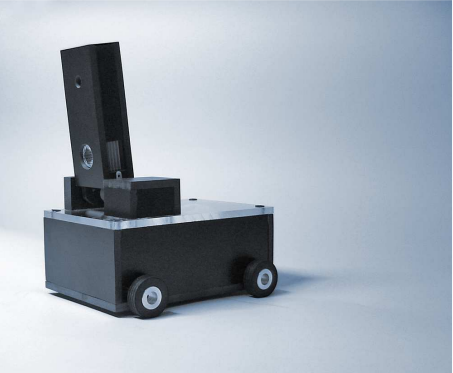
\includegraphics[height=110mm]{../images/ch04/de_side_view.png}
 \caption{Wygląd robota w pierwotnej konfiguracji po zmontowaniu wszystkich elementów}
 \label{fig:DESideView}
\end{figure}

Ze względu na dużą ilość czujników dodatkowych których obsługa została dodana w
obecnej wersji robota, wszelkie próby wykorzystania istniejącej obudowy
zakończyły się niepowodzeniem. Dlatego też zaprojektowany został ekspander
pozwalający w~łatwy sposób zintegrować poprzednią konstrukcję z zestawem nowych
czujników i urządzeń peryferyjnych. Wspomniany ekspander ma postać
prostopadłościanu wykonanego w całości z płyt bezbarwnej pleksi. 
Wszystkie elementy elektroniczne zostały rozmieszczone na~spodniej płycie
ekspandera, a potrzebne połączenia zostały wyprowadzone poprzez otwory z
gniazdami zainstalowanymi w miejscu podłączenia czujnika. Schemat projektowy
dolnej płyty ekspandera widoczny jest na rysunku \ref{fig:SensorsBoard}.

\begin{figure}[h!]
 \centering
 \subfloat[Wymiarowanie projektu
 obudowy]{\label{fig:SesnsorBoardA}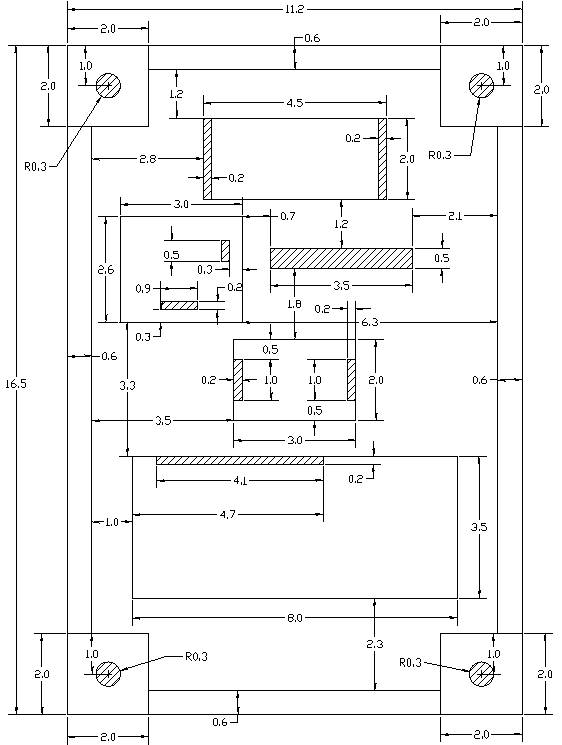
\includegraphics[width=0.535\textwidth]{../images/ch04/sensor_board.png}}
 \subfloat[Rozmieszczenie poszczególnych elementów wewnątrz
 obudowy]{\label{fig:SesnsorBoardA}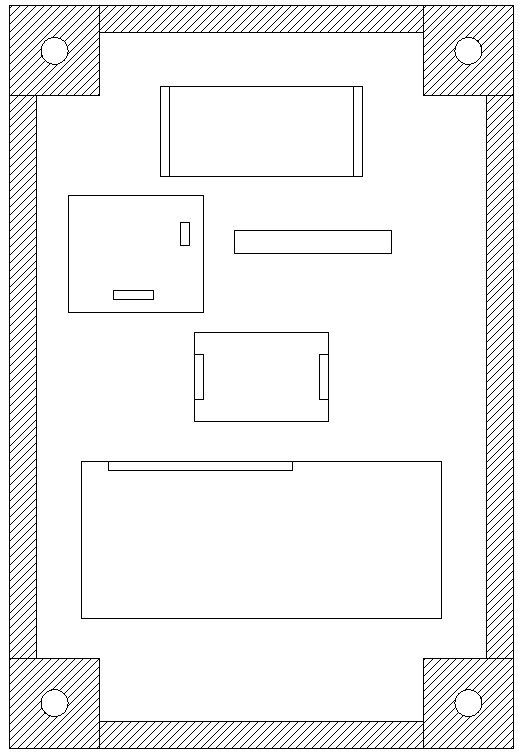
\includegraphics[width=0.465\textwidth]{../images/ch04/sensor_board_simple.png}}
 \caption{Projekt modułu rozszerzeń obudowy robota}
 \label{fig:SensorsBoard}
\end{figure}

W~centrum ekspandera umiejscowiony został żyroskop, celem takiego zabiegu było
wyeliminowanie potencjalnych problemów związanych z pomiarem kąta o jaki robot
się obrócił w przypadku gdy czujnik pomiarowy nie znajduje się na osi wzdłuż
której obrót jest dokonywany. W~południowej części umieszczony został
wyświetlacz LCD za pomocą którego użytkownik będzie mógł na bieżąco monitorować
aktualne działania robota. W~północnej części zamontowany został akcelerometr
oraz magnetometr. Taka konfiguracja pozwoliła na ograniczenie ilości i długości
przewodów potrzebnych do podłączenia wszystkich elementów do płyty głównej
robota. Do tak przygotowanej płyty dołączona została elektronika umożliwiająca
podłączenie wszystkich dodatkowych modułów. Szczegółowa prezentacja
elektronicznej części płyty głównej ekspandera zamieszczona została w rozdziale
\ref{ch:ExpanderChapter}. 

Całość obudowy została zaprojektowana w taki sposób
aby umożliwić bezproblemowe podłączanie i odłączenie nie tylko poszczególnych
czujników ale również całego ekspandera. Takie podejście do problemu nie
tylko nie ogranicza możliwości dalszego rozwoju, ale~umożliwia również swobodne
modyfikowanie zestawu podłączonych czujników, co~w~znaczącym stopniu
ułatwia dodawanie nowych modułów pomocniczych. Wygląd działającego ekspandera
dołączonego do pierwotnej budowy robota można zobaczyć na~zdjęciu~\ref{fig:DE2SideVIew}. 

\begin{figure}[h!]
 \centering
 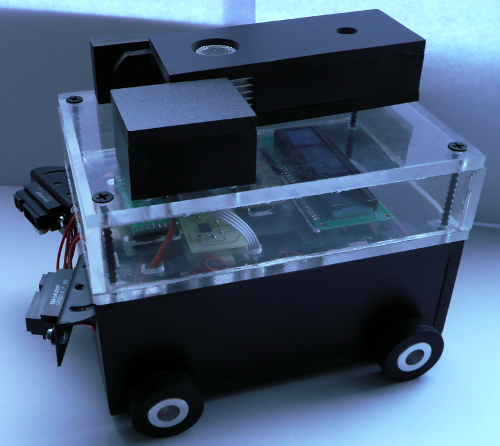
\includegraphics[height=125mm]{../images/ch04/de2_side_view.png}
 \caption{Wygląd robota z zamontowanym modułem rozszerzeń}
 \label{fig:DE2SideVIew}
\end{figure}